\documentclass{article}
\usepackage[utf8]{inputenc}
\usepackage{todonotes}
\usepackage{array}

\title{CSC470: Software Engineering Final Report\\ TESS: The Extraordinary Sudoku Solver}
\author{Team: \#1 \\David Koval and Joseph Mammo\\Instructor: Dr. Ahyoung Lee}
\date{ 4/24/17 \\ v1.1 }

 
\renewcommand*\contentsname{Table of Contents}

 
\begin{document}
 
\maketitle

\clearpage

\tableofcontents

\clearpage

\section{Summary} 
\todo{!!!} High level summar with 1 page. the project goals, motivation or problem issues (requirements). Design considerations and choices to solve the problems to achieve the goals. Implementation, validation and testing plans.


 
\section{Introduction}
 
Overall introduction
\subsection{Purpose}
\subsection{Scope}
\subsection{Definitions, acronyms, and abbreviations}

\begin{tabular}{ | m{8em} | m{24em}|  } 
\hline
\textbf{Term}& \textbf{Definition}  \\ 
\hline
DESC & Description  \\ 
\hline
Grid & This is where all the values are stored for the player to see.  \\ 
\hline
ID & Identification  \\ 
\hline
PW & Priority Weights  \\ 
\hline
User & Whoever will be using the app  \\ 
\hline
\end{tabular}

 

\section{Goals}

This is the goals section. 


 
\section{Specific Requirements}
This is the specific requirements section.

Be sure to include numbering scheme including Identifier (RQ1, RQ2, and RQn) and PW (the priority weights, may be the highest priority = 5 and the lowest priority = 1) to allow traceability.

Provide a high-level use case diagram for the high-level system models and a traceability matrix for the requirement validation.
 
\subsection{Functional Requirements}
\todo{How to add todo}
\textbf{ID:R1} \newline TITLE: Play Game Option\newline DESC: The user first opens up the app, they should be able to choose the option to play a Sudoku puzzle. They user should be able to stay as long as they want to on this screen.\newline PW: 3 \newline \newline
\textbf{ID:R2} \newline TITLE: Select Difficulty \newline DESC: The user should be able to select a difficulty setting that better suites needs at any time. There should be 5 difficulty options for the user to choose from. 1 being the easiest all the way down to 5 being the hardest.\newline PW: 2 \newline \newline
\textbf{ID:R3} \newline TITLE: Back Option \newline DESC: The user should be able to return to the main screen from the select difficulty screen if they don't select a difficulty. The user can remain on the select difficulty as long as the want to.\newline PW: 1 \newline \newline
\textbf{ID:R4} \newline TITLE: Continue Game \newline DESC: The user should be able to continue a game that has been previously started whether or not the app has been closed. All of the user's input should be saved so they could be brought up again should the user want to continue a game.\newline PW: 4 \newline \newline
\textbf{ID:R5} \newline TITLE: Get Puzzle \newline DESC: When the user selects a difficulty, a puzzle with the selected difficulty should be retrieved from the database for the user to be able to play it and enjoy the game.\newline PW: 2 \newline \newline
\textbf{ID:R6} \newline TITLE: Solver Option \newline DESC: On started, the user should be able to select the Solver option in the app to go straight to the solver part of the app. \newline PW: 5 \newline \newline
\textbf{ID:R7} \newline TITLE: Input Sudoku Puzzle To Solve \newline DESC: The user needs to be able to input any sort of Sudoku puzzle that the user has, with or without any extra numbers the user wishes to input. \newline PW: 5 \newline \newline
\textbf{ID:R8} \newline TITLE: Check Current Board \newline DESC: The user should be able to check the status of the current puzzle they are working on. The user should be able to view the inputs that are conflicting with each other. They should be marked in some way for the user to be able to see them clearly. \newline PW: 4 \newline \newline
\textbf{ID:R9} \newline TITLE: Delete an Input Value \newline DESC: The user should be able to delete an input value that they put in previously or a value that the system put in automatically. \newline PW: 5 \newline \newline
\textbf{ID:R10} \newline TITLE: Clear Board \newline DESC: The user should be able to clear the entire board easily and effortlessly. \newline PW: 3 \newline \newline
\textbf{ID:R11} \newline TITLE: Solve Current Board \newline DESC: The user should be able to have the option to solve the current board that they are working on. It should use the input the system put in as well as the inputs the user decided to add. \newline PW: 5 \newline \newline
\textbf{ID:R12} \newline TITLE: Play Sudoku Game \newline DESC: The user should be able to play a Sudoku game by selecting certain boxes and input a value into them. \newline PW: 4 \newline \newline
\textbf{ID:R13} \newline TITLE: Hint Option \newline DESC: The user should have the option to get a hint on the current Sudoku game they are playing. The hint should display any correct value on the given board. \newline PW: 1 \newline \newline
\textbf{ID:R14} \newline TITLE: Download Mobile Application \newline DESC: The user should be able to download the mobile application either from the Play Store or via Email to their Android phone. The download should be free. \newline PW: 5 \newline \newline




\subsection{Non-Functional Requirements} 

\textbf{ID:RQ1} \newline TITLE: System Availability \newline DESC: The system needs to  be available to the user 99.9\% of the time, whether or not the system is being used. The system can only be down for 0.1\% of the time for updates or maintenance. \newline \newline
\textbf{ID:RQ2} \newline TITLE: Solve Time \newline DESC: The app should be able to solve a given Sudoku puzzle, whether there is or isn't a solution in under 5 seconds.\newline \newline
\textbf{ID:RQ3} \newline TITLE: Search Algorithm \newline DESC: The Suduko solver must utilize some search algorithm such as depth first search or breadth first search or any other searching algorithm. \newline \newline
\textbf{ID:RQ4} \newline TITLE: Pruning Technique \newline DESC: There must be some sort of pruning technique with solving the problem because 9\textsuperscript{81} is not feasible. \newline \newline
\textbf{ID:RQ5} \newline TITLE: Database Storage \newline DESC: The Database needs be stored locally on the device and new puzzles should be added to the device through updates or pulled from an external database. \newline \newline
\textbf{ID:RQ6} \newline TITLE: Easy to Use \newline DESC: The app should be very simple to use to any player with some general idea of how Sudoku puzzles work. \newline \newline
\textbf{ID:RQ7} \newline TITLE: Private Information \newline DESC: The app should not keep any personal information about the user. There app should not ask the user for any passwords. \newline \newline

\subsection{System Model}

\subsubsection{Actors}

\begin{itemize}
   \item Player: This is the primary actor who will be using the app.
   \item Database: This is the datastore that on the device that contains all the Sudoku puzzles for the user to play.
\end{itemize}

\subsubsection{Use Cases}

\textbf{ID:UC1} \newline TITLE: Select Play Game \newline ACTORS: Player \newline DESC: Player opens up the app and selects to play a Sudoku puzzle. \newline \newline
\textbf{ID:UC2} \newline TITLE: Select Solver \newline ACTORS: Player \newline DESC: Player opens up the app and selects the Solver option to solve a Sudoku puzzle they might have. \newline \newline
\textbf{ID:UC3} \newline TITLE: Selects a difficulty \newline ACTORS: Player and Database\newline DESC: Player selects a difficulty from the options available and a Sudoku board is filled with a puzzle similar to the difficulty the Player selected. \newline \newline
\textbf{ID:UC4} \newline TITLE: Quitting Time \newline ACTORS: Player and Database \newline DESC: When Player decides to quit the puzzle they are currently working on, the puzzle is saved to the database so Player can continue playing it.  \newline \newline
\textbf{ID:UC5} \newline TITLE: Selecting Continue \newline ACTORS: Player and Database \newline DESC: When Player decides to play a game again and selects the continue option to bring up the previously saved game they were playing. \newline \newline
\textbf{ID:UC6} \newline TITLE: Hint Option \newline ACTORS: Player \newline DESC: The Player is unsure of any other moves, so Player decides to select the hint option in order to recieve a hint about the current Sudoku puzzle they are working on. \newline \newline
\textbf{ID:UC7} \newline TITLE: Solve Option \newline ACTORS: Player \newline DESC: The Player is tired of playing and wants to see the solution to the Sudoku puzzle, so they decided to tap the solve button to get all the answers. \newline \newline

\subsubsection{Use Case Diagram}
\subsubsection{Prototyping}
\subsubsection{Traceability Matrix}
\section{System Design}
This is the system design section.

\subsection{Desgin Overview}
Provide an overview of the design, including diagrams, key design subsections, and how they relate or connect to one another (e.g., Interaction, structural models).

\subsection{Realistic Constraints and Professional Standards}
Identify and discuss realistic constraints on the problem, such that constraints may include economic, environmental, social, ethical, health and safety, manufacturability, policy issues, etc.
\subsubsection{Constraints}
\textbf{ID:C1} \newline TITLE: Memory Space \newline DESC: The app should have a small footprint. The entire app should take up less than 5MBs of memory, this is including with future updates as well.\newline\newline
\textbf{ID:C2} \newline TITLE: Internet Connection for Updates\newline DESC: The app must have an internet connection established to be able to retrieve updated information from a master database. \newline\newline
\textbf{ID:C3} \newline TITLE: Programming Language \newline DESC: The app must be written in mainly Java, there may be other languages within the program, but the main part of it should be in Java.\newline\newline
\textbf{ID:C4} \newline TITLE: Android Device Only \newline DESC: The system must work on Android Devices, specifically the Galaxy Note 5 first, the following versions will include other phone models.\newline\newline
\textbf{ID:C5} \newline TITLE: Time to Solve \newline DESC: The app should take less than 5 seconds to output the solved Sudoku puzzle or report that it can't be solved.\newline\newline
\textbf{ID:C6} \newline TITLE: Database Usage \newline DESC: The app must utilize some sort of database to hold the stored puzzles.\newline\newline

\begin{figure*}[!t]\centering
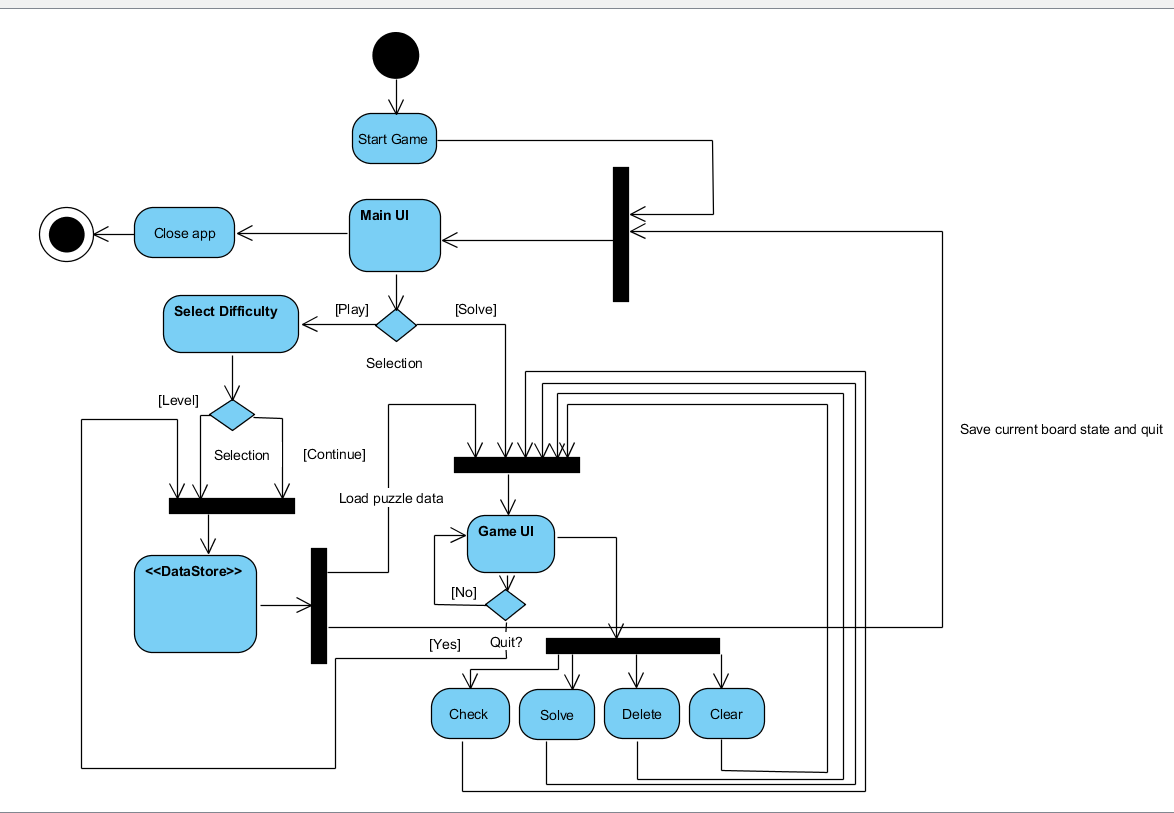
\includegraphics[width=6.0in]{./Figure/Activity_Diagram.PNG}
\caption{Activity diagram of a system.}\label{fig:act_dia_1}
\end{figure*}


\subsection{Alternative Designs and Design Choices}
Describe alternative designs that were considered during execution of the project. Discuss how design choices were guided by constraints and other factors. E.g., architectural design models – Layered or Client-server and details shown using activity diagram as shown in Figure \ref{fig:act_dia_1} (Context model), sequence diagram (Interaction model), class diagram (Structural model).

\begin{figure*}[!t]
	\centering
	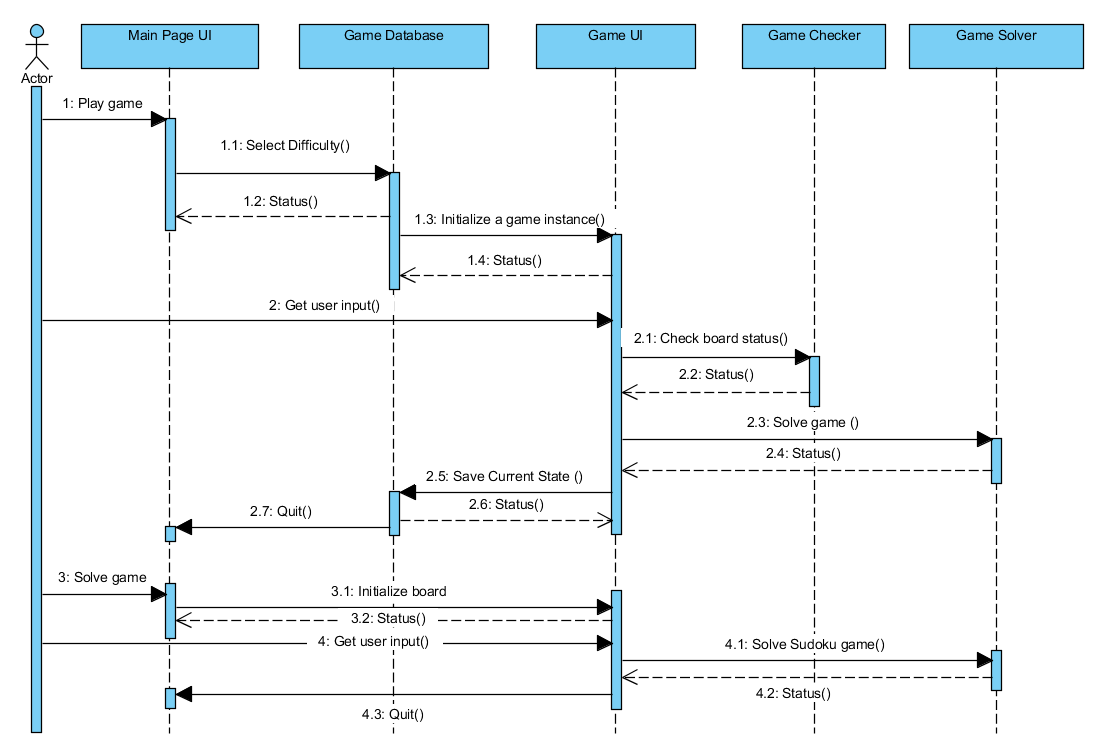
\includegraphics[width=6.0in]{./Figure/Sequence_Diagram.PNG}
	\caption{Sequence diagram of a system.}
	\label{fig:act_dia_2}
\end{figure*}


\section{System Implementation}
This is the system inplementation section.

Describe the technical details for each of the subsystems or a the system-level and
provide sequence diagrams or station/activity diagrams for your system implemenation.



\section{System Testing}
This is the system testing section.

\subsection{Test Plan}
Provide your test plan with unit testing (Black-box testing and White-box testing), integration testing (Top-down or bottom-up approach) and system testing.

\subsection{Test Results}
Show your test restults and evaluate them. 

\section{Conclusions}
This is the conclusions section.

Overall summary of design methodologies, key creative approaches and potential
contribution/impact. \cite{hahahaha}

\bibliographystyle{IEEEtran}
\bibliography{Bibliography}


 
\end{document}